\documentclass[a4paper,12pt]{article}
%\usepackage[utf8]{inputenc}
\usepackage[english]{babel}
\usepackage[scaled=.98]{courier}
%\usepackage{microtype}
\usepackage{graphicx}
\usepackage[table,xcdraw]{xcolor}
\graphicspath{ {./images/} }
\usepackage{wrapfig}
\usepackage{xcolor}
\usepackage{enumitem}
\usepackage{fancyhdr}
\usepackage{amsmath}
%\usepackage[a4paper,inner=1.7cm, outer=2.7cm, top=2cm, bottom=2cm, bindingoffset=1.2cm]{geometry}
\usepackage{blindtext}
\usepackage{index}
\usepackage{hyperref}
\makeindex

%\renewcommand{\familydefault}{\sfdefault}

\begin{document}

\begin{figure}
    \centering

\includegraphics[width=4.5cm]{logo.jpg}    
\end{figure}

\begin{titlepage} % Suppresses headers and footers on the title page

	\centering % Centre everything on the title page
	
	\scshape % Use small caps for all text on the title page
	
	\vspace*{\baselineskip} % White space at the top of the page
	
	%------------------------------------------------
	%	Title
	%------------------------------------------------
	
	{\color{blue} \rule{\textwidth}{1.6pt}\vspace*{-\baselineskip}\vspace*{2pt} }% Thick horizontal rule
	{\color{blue} \rule{\textwidth}{0.4pt} } % Thin horizontal rule
	
	\vspace{0.75\baselineskip} % Whitespace above the title
	
	{\Large \textbf{SCHOOL\\ MANAGEMENT \\ \vspace{0.25cm} SYSTEM}   } % Title
	
	\vspace{0.75\baselineskip} % Whitespace below the title
	
	{\color{blue} \rule{\textwidth}{0.4pt}\vspace*{-\baselineskip}\vspace{3.2pt} }% Thin horizontal rule
	{\color{blue} \rule{\textwidth}{1.6pt} }% Thick horizontal rule
	
	\vspace{2\baselineskip} % Whitespace after the title block
	
	%------------------------------------------------
	%	Subtitle
	%------------------------------------------------
	
	%\textbf{\normalsize Lab Instructor - Nazmul Alam Diptu \\ Course Instructor - Tarek Ibne Mizan}% Subtitle or further description
	{\scshape\large  Lab Instructor - Nazmul Alam Dipto \\Course Instructor - Tarek Ibne Mizan \\}
	
        \vspace*{\baselineskip} % Whitespace under the subtitle
	
	%------------------------------------------------
	%	Editor(s)
	%------------------------------------------------
	
	\huge\underline{Project Report By} 
	
	\vspace{0.5\baselineskip} % Whitespace before the editors
	
	{\scshape\large \textbf{Akif Zahin - 2131865042 \\ Mohammed Aman Bhuiyan - 2131864642 \\ Tabassum Bari - 2132177642 \\} } % Editor list
	
	\vspace{0.5\baselineskip} % Whitespace below the editor list
	
	\textit{\large \textbf{North South University }  } % Editor affiliation
	
	\vfill % Whitespace between editor names and publisher logo
        
        
	%------------------------------------------------
	%	Publisher
	%------------------------------------------------
	
	
	
        
        \vspace{-1em}
        \small {CSE215.12L - GROUP 3 - 2022} % Publisher
         
         \vspace{0.3\baselineskip} % Whitespace under the publisher logo

\end{titlepage}

\tableofcontents
\vspace{3cm}
\begin{center}
    \large For Github Repository - Click \href{https://github.com/akifzahin/CSE215.12L-Group-3-School-Management-System}{\textbf{HERE}} 
\end{center}

\newpage

\section{Tables}
\enlargethispage{\baselineskip}
Please see the table shown below:- 
\begin{itemize}
    \item \hyperref[sec:projsec]{Figure 1.1 - Table for Man Hours worked}
\end{itemize}

\section{Introduction}
\enlargethispage{\baselineskip}
A school management system is a large collection of programs which incorporates information handling and connects them to systems that save data from its users, where it saves the hassle of manual record-keeping by making our daily lives more faster then we had ever imagined. The system is especially adept in storing huge amounts of data that can easily be accessed, edited or deleted as according to the user type. \par In this age of modern urbanization, schools and educational institutions have always been demanding a solution for that makes their administration more clean. This is where the school management system comes in action.

\subsection{About NSHS School Management System}
\enlargethispage{\baselineskip}
The project, North South High School Management System, serves to give us a glimpse of how useful a well implemented management system can be and how important it is for schools to adopt it into their hectic administration organization.
\par With graphical user interfaces for the admin, teachers and students, we can easily access different files which we can then access or edit with the click of a button. Moreover, entities can also access each other to create a more dynamic approach in terms of accessing information.

\subsection{Purpose of System}
\enlargethispage{\baselineskip}
The purpose of this system is demonstrate the use of record keeping through easy to use software that increases efficiency by decreasing our time spent writing on paper. \par It is also useful in creating effective solutions for the administration to monitor teachers and students and their respective positions in the classroom. Individual classrooms can be created to add more teachers and students by the admin who can view and access everything in the system.
\newpage

\subsection{Benefits of System}
\enlargethispage{\baselineskip}
\begin{itemize}
    \item It saves valuable time by creating faster approaches towards data storage and record keeping
    \item It closes the communication gap between the different entities
    \item It helps give new life to archaic methods for authorities such publishing grades or attendance
    \item It handles the lifetime data of students to keep track of a child's daily activities 
    \baselineskip
    \item It gives parents a new way to monitor their child through an easy approach thus improving communications
\end{itemize}


\subsection{Features of System}
\enlargethispage{\baselineskip}
\begin{itemize}
    \item Teacher Management - Teachers can login into their homepage to publish grades, give attendance to a particular student or get their information stored in file by searching their names. They can also view their own information or view their fees as required
    \item Academic Management - This includes the ability that teachers have to assign different grades to each student while also assigning them their attendances.
    \item Student Management - Students can login into their homepage to be limited to viewing their personal information, their grades,their attendance and their fees. However, they can also write anonymous teacher reviews which are not accessible by anyone except for the admin.
    \item Admin Management - The Admin has master control over the whole system as it can access a teacher or student database where every entity information can be accessed by them in a clean and organized manner. They can also search a particular teacher or student to see their respective information. \par Most importantly, they can also add or delete an entity(teacher or student alike) from the system given the need which gives him the most power.
    \item File Management - The system consists of text files which stores the login data for students and teachers which is also used to verify the data. Each time a user registers, a text file is appended for the teachers or students which serves as a database. 
\end{itemize}
\newpage
\section{User Cases and Examples}
\enlargethispage{\baselineskip}
This section provides of the three main entities interacting with the system and how the system can react to their needs.

\subsection{Use Case - 1}
\enlargethispage{\baselineskip}
John Doe Jr., a student of Class 8 in North South High School is interested in viewing his assigned grades as he is anxious. He has a few options:- 
\begin{enumerate}
    \item He can login to his account.
    \item He can click on a button that will access his file, saved by the teacher and show him his result.
    \item He can also see his attendance the same way.
    \item If he wishes he can check on his fees or his personal information.
   \baselineskip
   \item  He can even write a teacher review at the end of the school year.
\end{enumerate}  


\subsection{Use Case - 2}
\enlargethispage{\baselineskip}
Mrs Jane Doe, a junior teacher in North South High School has been tasked by the Dean to use the new system and assign the grades and attendance to the respective students. She has a few options:- 
\begin{enumerate}
    \item She can then create an account and register her information
    \item she will be able to access individual student files by searching up their names and assigning the result and the attendance to their files, one by one.
    \item  She can the also view individual student data.
    \item She can see her fees or her own personal information. 
\end{enumerate}  
\newpage

\subsection{Use Case - 3}
\enlargethispage{\baselineskip}
The Admin, who has master control over the program can login to the system and be presented with a variety of different options:-
\begin{enumerate}
    \item He can add students or teacher to the classroom, which acts as a repository of data.
    \item He can delete teachers or students, where their individuals file will be deleted along with the auto update of the classroom.
    \item He can search individual entities to keep track of particular students and their information.
    \item He can see the student or teacher database to see all the user information stored in the system.
    \item He can view the teacher reviews written by the students which will still be anonymous.
\end{enumerate}
\newpage
\subsection{Limitations}
\begin{itemize}
    \item The lack of a dedicated database system means information cannot be edited in this system by the admin
    \item The system is not dynamic since current methods cannot access specific user files and auto updated the interfaces to match with the current user
    \item Options limited to only view fees or salaries since integration of online banking system is absent
    \item Security risk is evident since there is no encryption available in this particular prototype
    \item User interfaces can be interpreted as dated and old since the lack of a dedicated front-end system can make things less responsive
\end{itemize}

\section {Program Breakdown}
\enlargethispage{\baselineskip}
This section describes the technologies and assets used to build the project from the ground up.

\subsection{Front-End Development}
\enlargethispage{\baselineskip}
There are in total, 28 Graphical User Interfaces used in this project. Some few examples include:-
\begin{itemize}
    \item Welcome Page
    \item Student Home Page
    \item Teacher Home Page
    \item Admin Home Page
    \item Teacher Registration and Login Page
    \item Student Registration and Login Page
\end{itemize}
\newpage

\subsection{Back-End Development}
\enlargethispage{\baselineskip}
\begin{enumerate}
   
   \item \textbf{Account Creation and Login}
    \begin{enumerate}
        \item Writing Login Data in Files for Data and Verification
        \item Registration Forms which save data by Serialization    
    \end{enumerate}
   
   \item \textbf{Profile Management and Homepage Functions}
    \begin{enumerate}
        \item View Information
        \item Publish Grades and Give Attendance
        \item Teacher Review 
        \item Add or Delete Student and Teachers
    \end{enumerate}
   
   \item \textbf{Searching Functions}
    \begin{enumerate}
        \item Search Students
        \item Search Teachers
        \item View Teacher Review
        \item View Student Database
        \item View Teacher Database
    \end{enumerate}

\end{enumerate}

\subsection{Tools and Technologies}
\enlargethispage{\baselineskip}

\begin{enumerate}
    \item Java Swing for Graphical User Interfaces
    \item Eclipse IDE and WindowBuilder 
    \item Git for Version Control
    \item Draw.io for UML Diagrams
    \item LaTex for Project Proposal and Report
\end{enumerate}
\newpage

\section{Importance of System}
\enlargethispage{\baselineskip}
\begin{enumerate}
    \item It helps the school and institution get accustomed to technologies in a non-overwhelming and easy way.
    \item It provides a way for user to effectively interact with each other.
    \item It provides the authorities to automatically manage student or teacher information during any changes.
    \item The school can remove their methods of taking attendance in heavy books since attendance is now more robustly set in the system.
    \item It reduces the cost of buying paper and record books.
\end{enumerate}



\section{Project Schedule}
\label{sec:projsec}
\enlargethispage{\baselineskip}
\begin{center}
    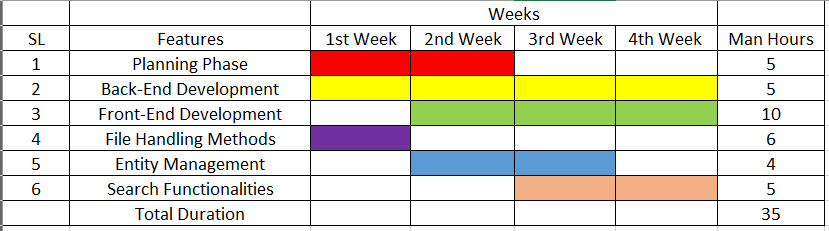
\includegraphics[width=15.2cm]{6.png}
    Figure 1.1 - Table showing Man Hours worked for the Month of July
\end{center}


\newpage


\section{Prototype Screenshots}
\enlargethispage{\baselineskip}
\begin{center}
    

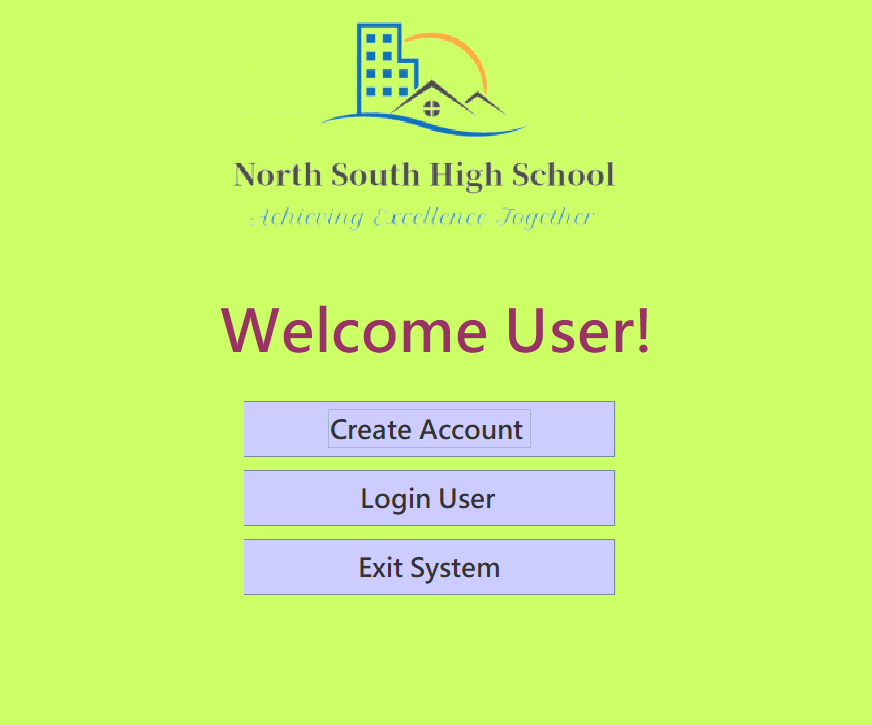
\includegraphics[width=9.2cm]{1.png} 
\\
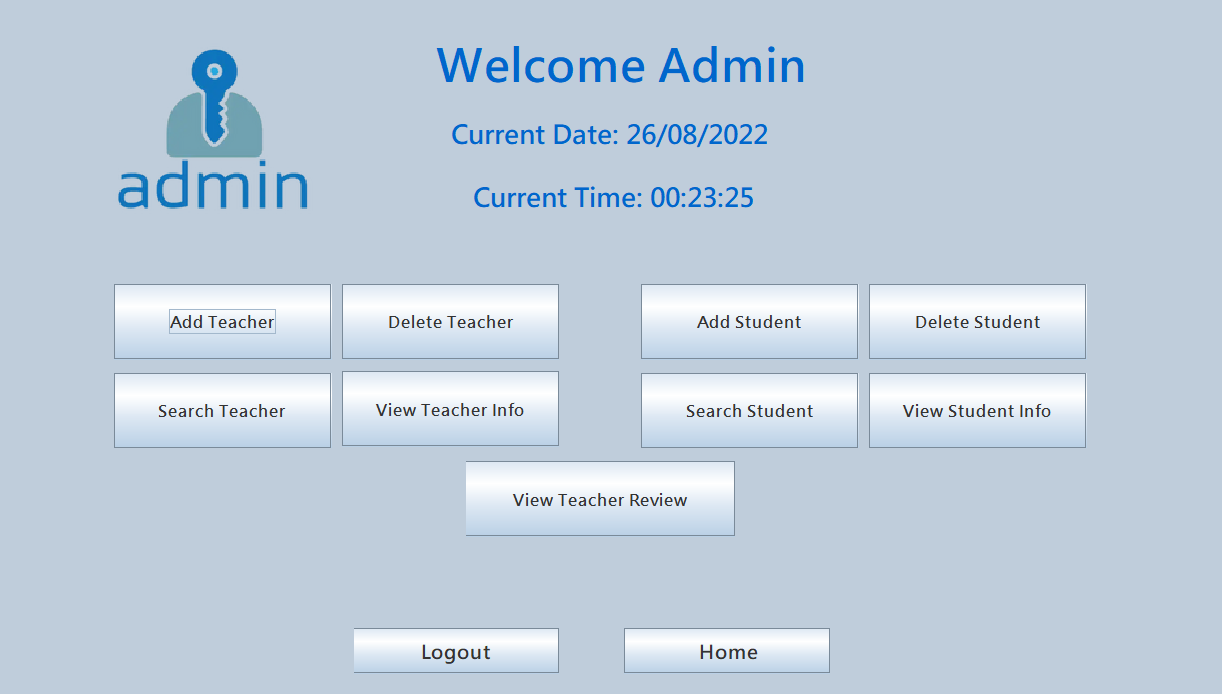
\includegraphics[width=9.2cm]{2.png} 
\\
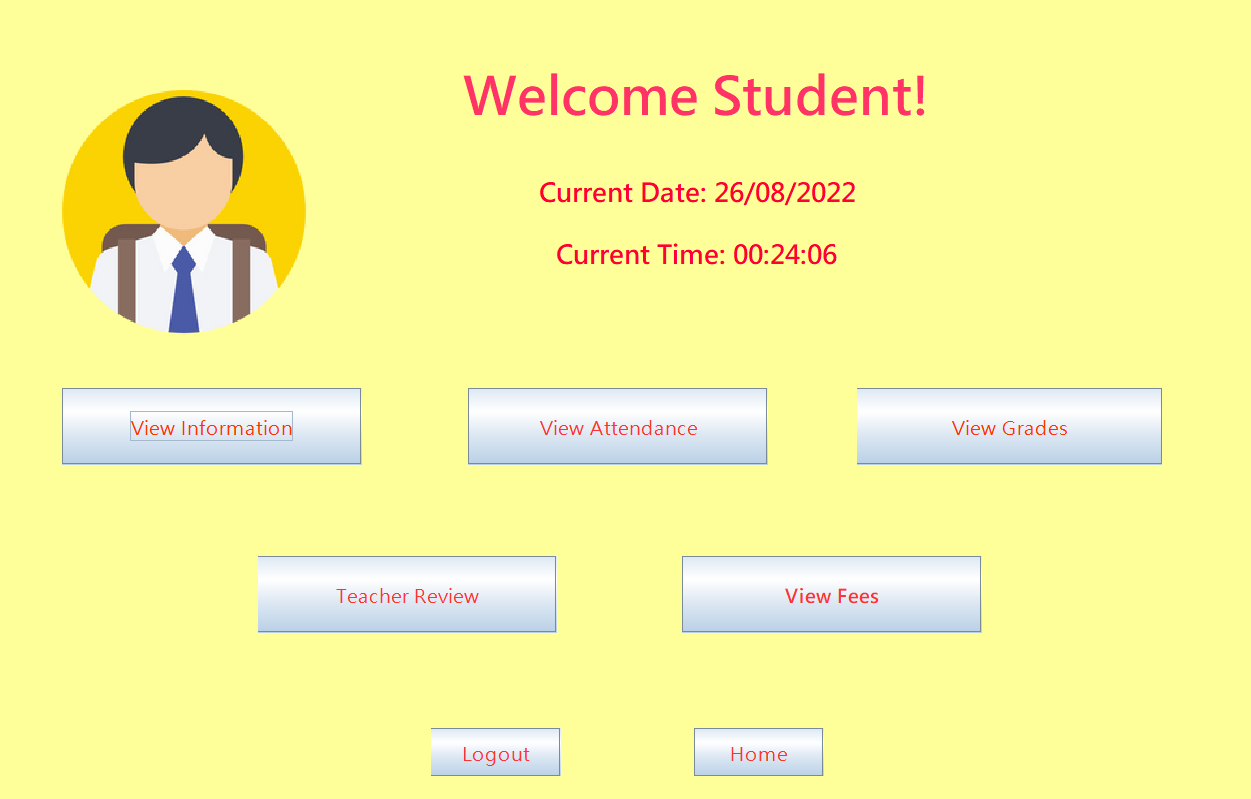
\includegraphics[width=9.2cm]{3.png} 
\\
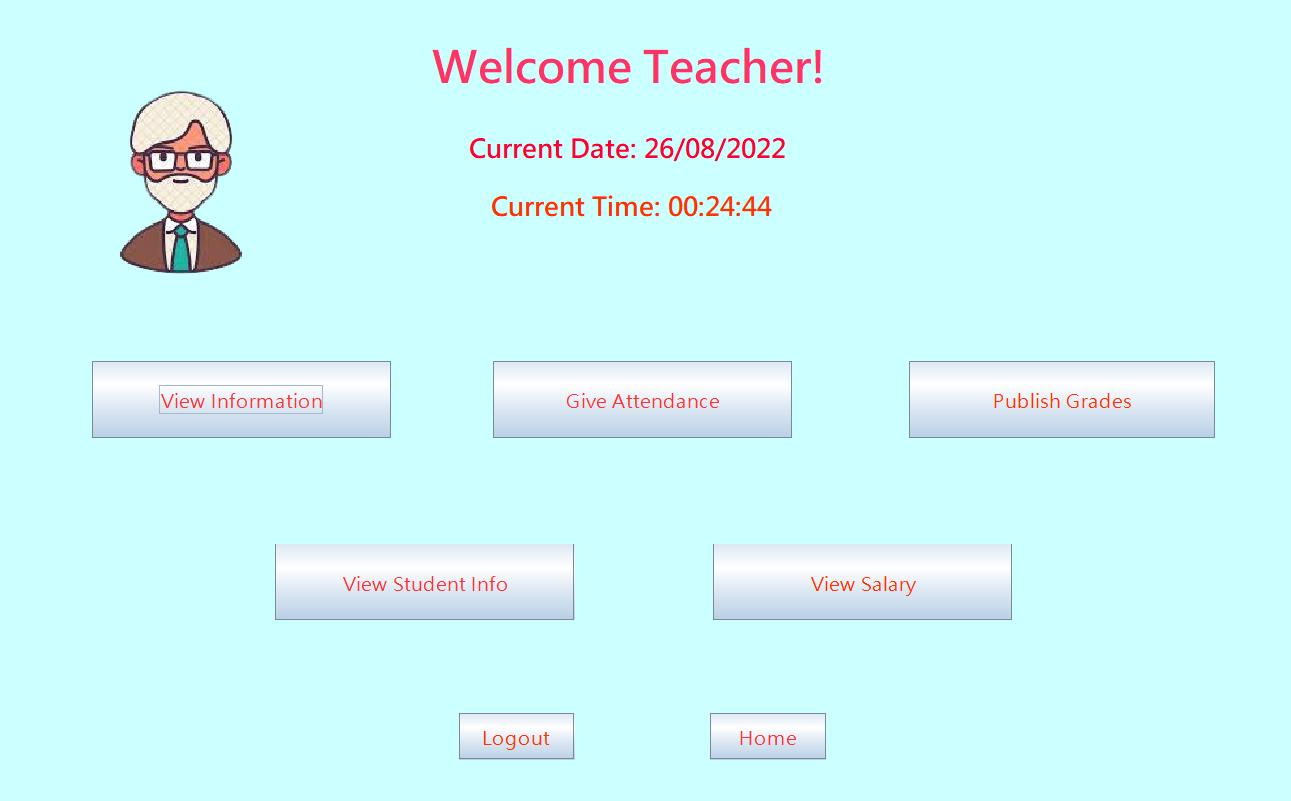
\includegraphics[width=9.2cm]{4.png}
\\
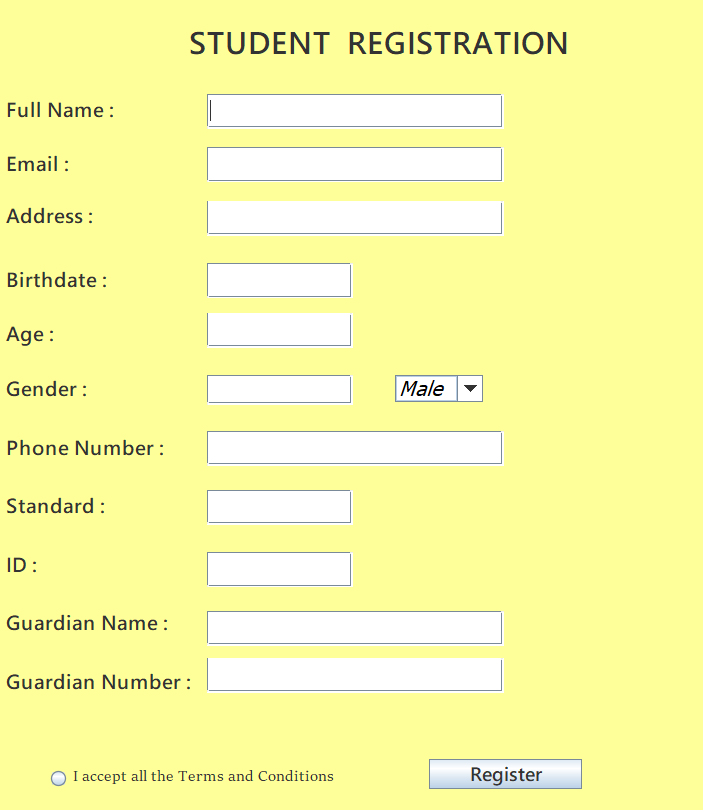
\includegraphics[width=9.2cm]{5.png} 
\end{center}
\newpage

\section{Final UML Diagrams}
This section contains the final UML Diagrams for the project.
\subsection{Class Diagram}
\begin{center}
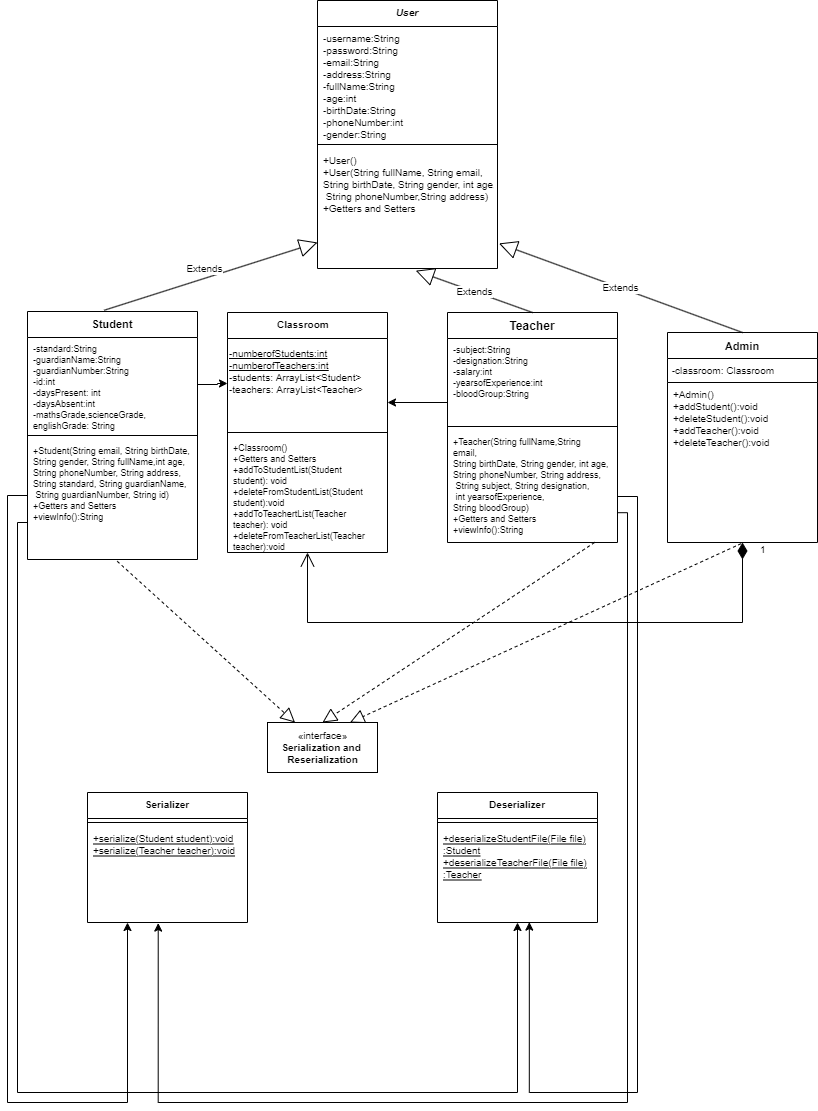
\includegraphics[width=11.2cm]{7.png} 
\end{center}
\newpage

\subsection{Sequence Diagram}
\begin{center}
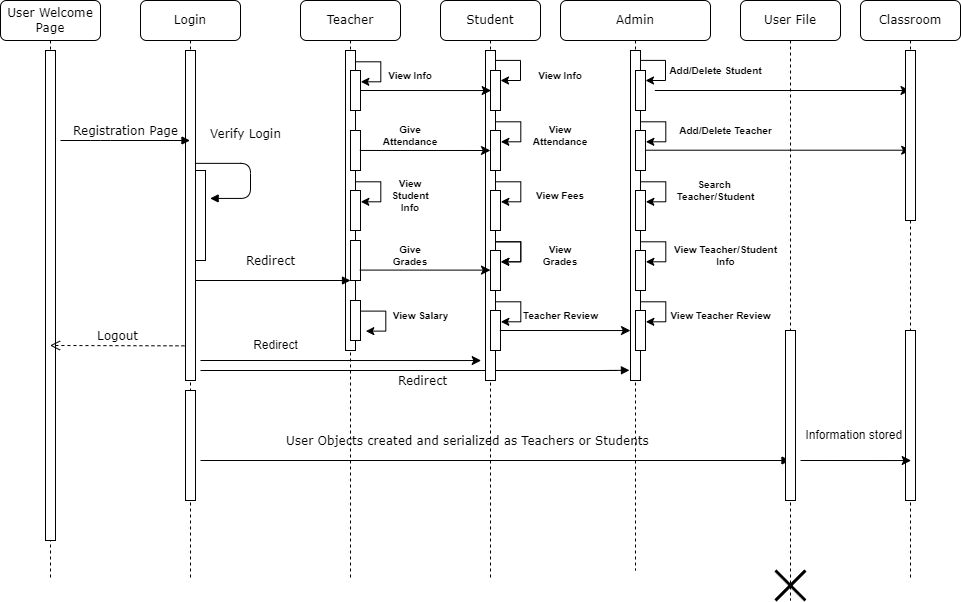
\includegraphics[width=11.2cm]{8.png} 
\end{center}
\newpage

\subsection{Use Case Diagram}
\begin{center}
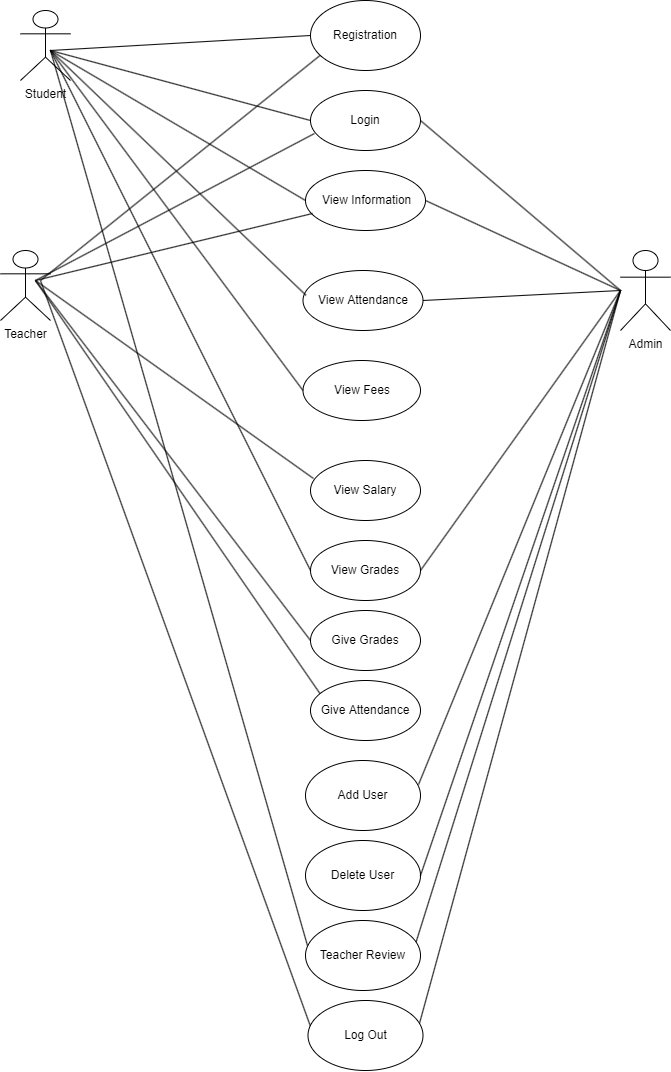
\includegraphics[width=11.2cm]{9.png} 
\end{center}
\newpage

\section{Conclusion}
\enlargethispage{\baselineskip}
In recent years, with the current pace of technological development, people have become
more and more demanding in terms of quality. The school authorities in
recent years have been looking forward to improve their student's performances in their school, where they obtain the highest percentage of knowledge and experience by interacting more with technology. This idea became more popular in the aftermath of COVID-19 period since more people were stuck home. Educational institutions therefore have become more reliable on management systems to conduct their daily tasks where, people under the system are highly benefited and can work without any hassle. This therefore became our ultimate goal, to bring forward a solution to change the current standards, and hopefully, make it better.   
\section{About Us}
This was project was created by Group 3 of CSE215.12L under the supervision of \textbf{Nazmul Alam Dipto}, Lab Instructor. The team consists of:-
\begin{enumerate}
    \item Akif Zahin 2131865042 - \href{https://github.com/akifzahin}{\textbf{Github Profile}}
    \item  Mohammed Aman Bhuiyan 2131864642 - \href{https://github.com/Aman554-EQ}{\textbf{Github Profile}}
    \item Tabassum Bari 2132177642 - \href{https://github.com/TabassumBari}{\textbf{Github Profile}}
\end{enumerate}

\begin{center}
 \large For Github Repository - Click \href{https://github.com/akifzahin/CSE215.12L-Group-3-School-Management-System}{\textbf{HERE}} 
\end{center}

\enlargethispage{\baselineskip}

\end{document}